\documentclass[5pt]{article}
\usepackage{array}
\usepackage{listings}
\usepackage{graphicx}
\usepackage{color}
\usepackage{hyperref}
\usepackage{caption}

\lstset{
  basicstyle=\fontfamily{lmvtt}\selectfont\small,
  columns=fullflexible,
}
\title{Rapport de la semaine du 11 avril 2022}
\author{TUELEAU Tom}
\begin{document}
\maketitle
\section{Introduction}
Ce document à pour objectif de faire l'états d'avancement du stage. Cellui-ci résumera donc le travail effectue la semaine du 11 avril 2022.
Je vous présente dans un premier temps mon instalation et comment j'ai aménager mon espace de travail. Dans une deuxiéme partie
nous verrons le travail que j'ai effectuer sur les capteurs et le microcontroleurs lors des 5 jours. Enfin, une dernier partie introduira le travail 
que je prévois d'effectuer lors des semaines à venir. 

\section{Instalation}
Lors de cette semaine j'ai pus m'installer aux niveaux du rucher. J'y ai apporté du matériel récupéré à l'iut (oscilloscope, shield ethernte pour
arduino uno) et du matériel personnel (arduino, capteurs, cable ...). Nous avons aussi à disposition un switch relier à la fibre. J'ai été, et je serais,
de nouveau amener à me déplacer à béziers pour deux raissons. La premier, afin de récurpérer du materiel et la seconde car le laboratoire à béziers est beaucoup
plus confortable pour manipuler des systemes electroniques.

\begin{center}	
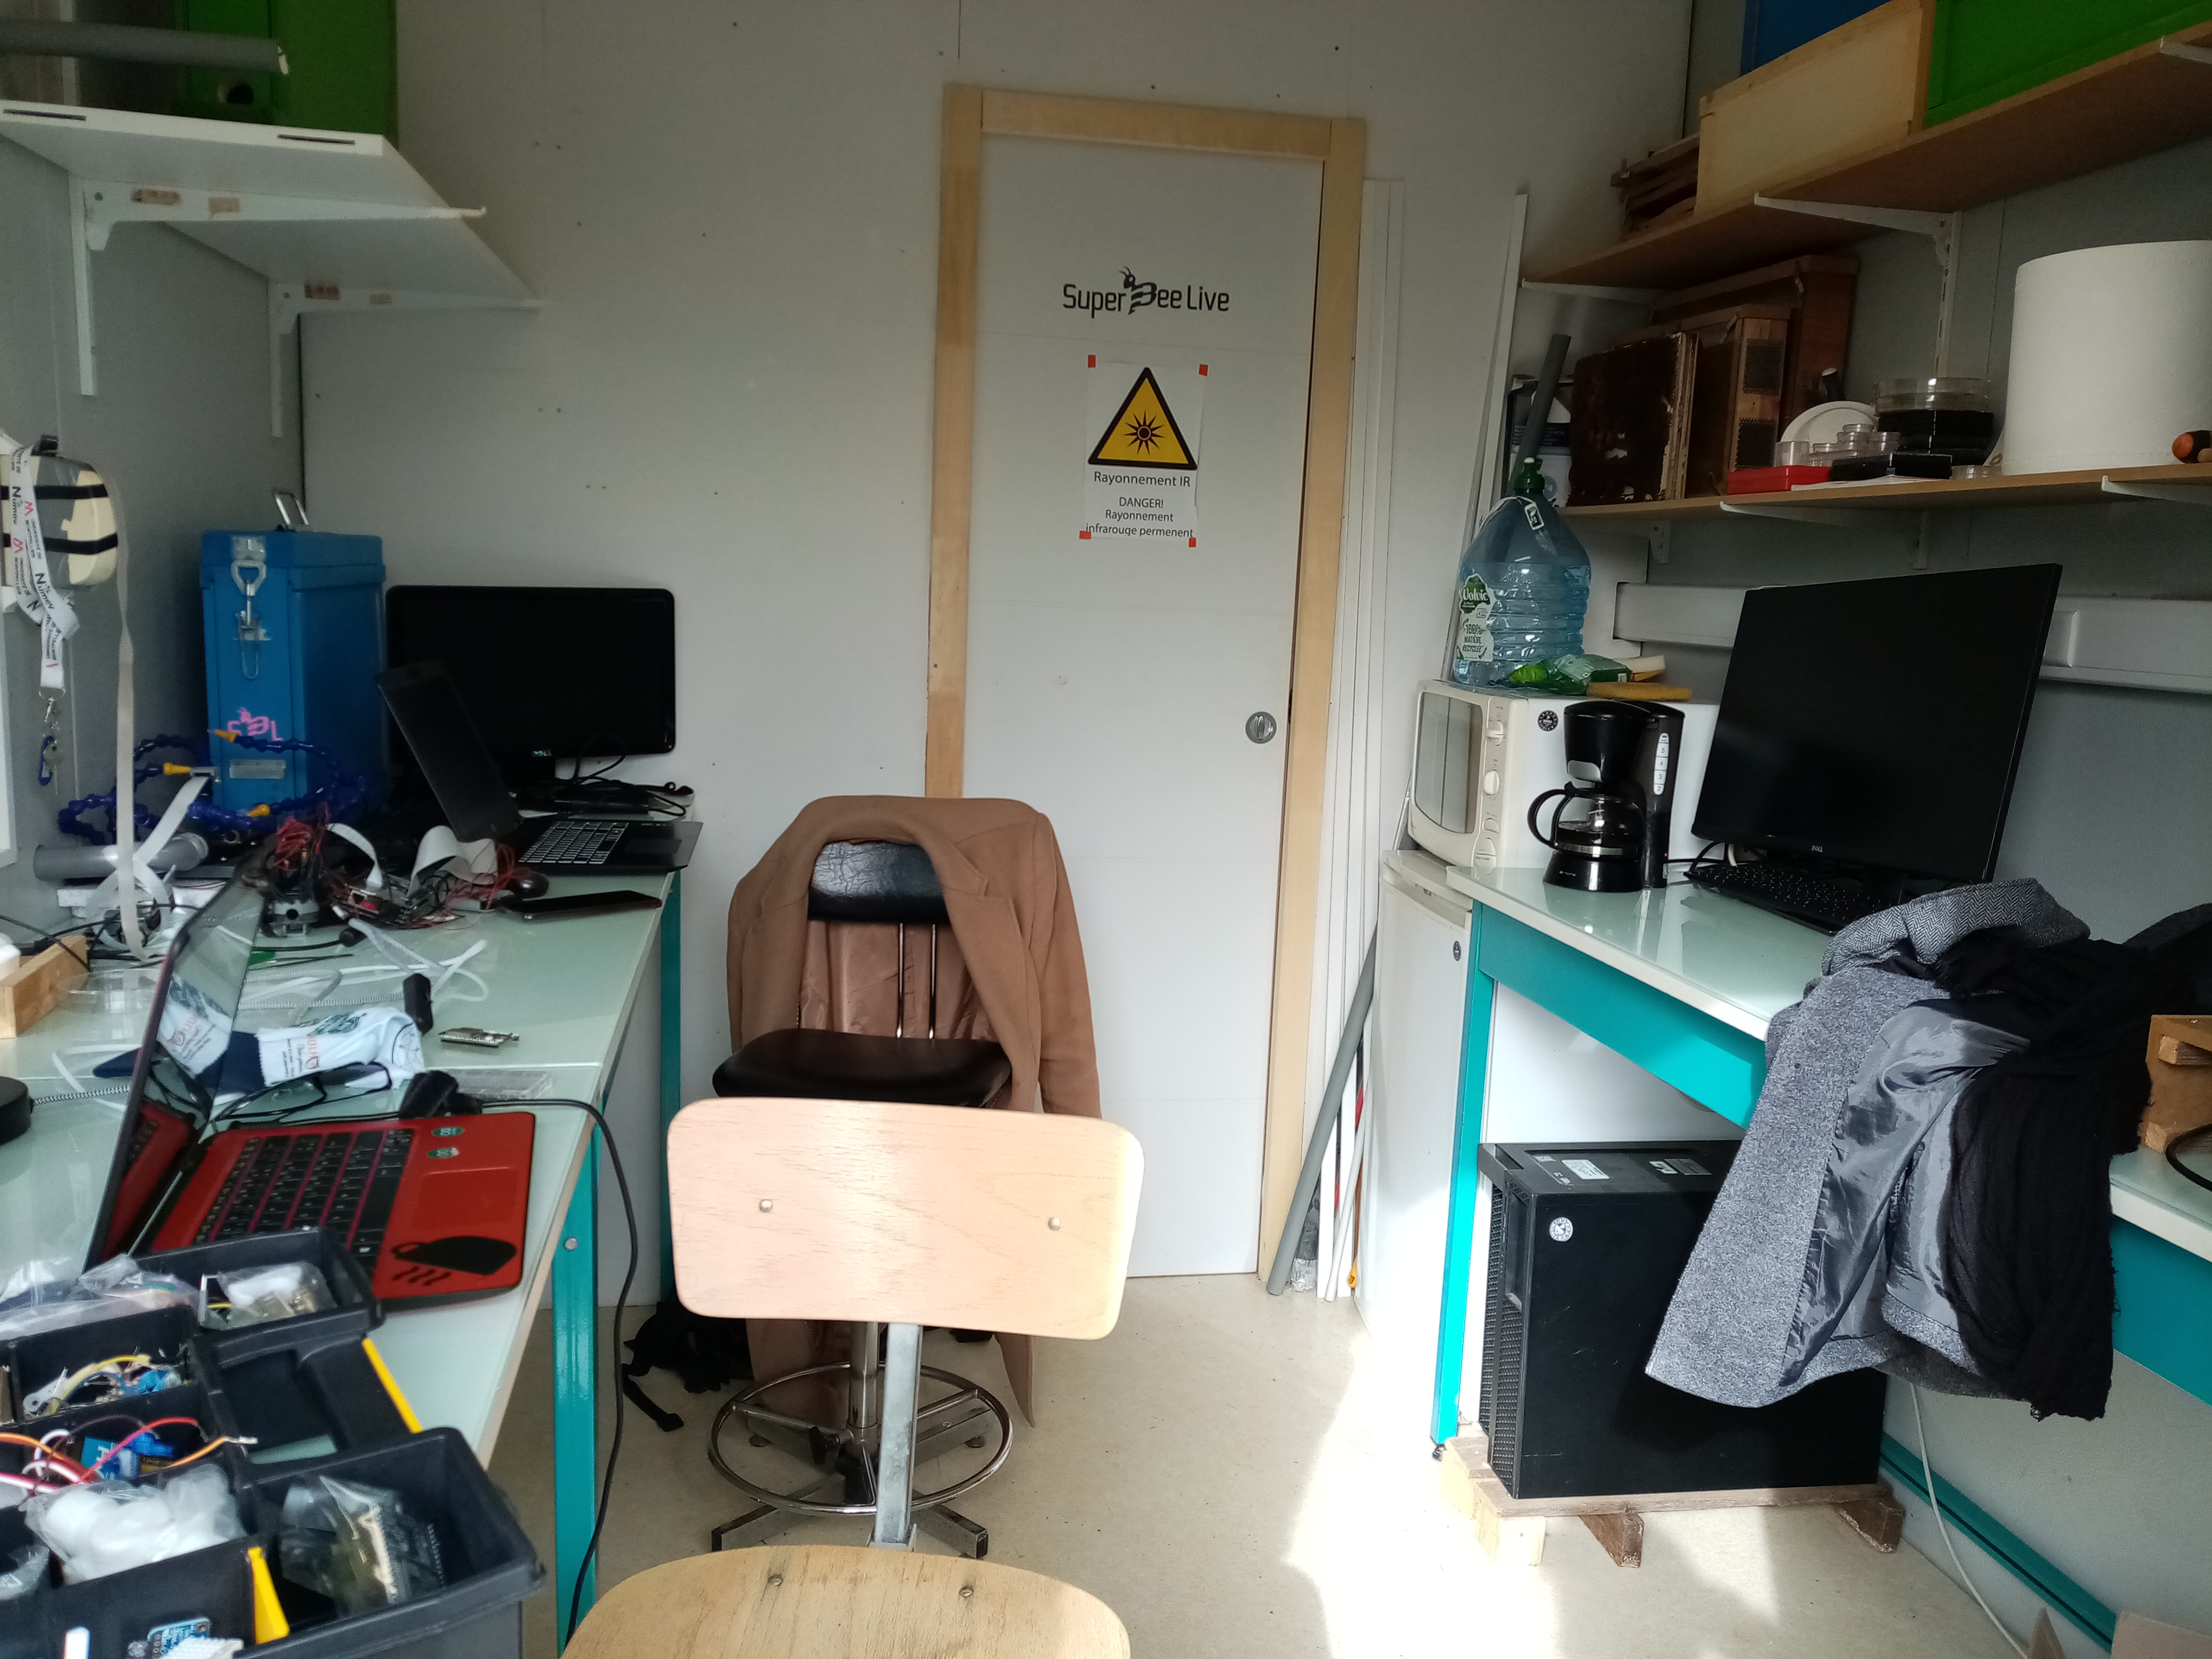
\includegraphics[scale=0.08]{interieur_rucher.jpg}
\captionof{figure}{Interieur du rucher}
\label{image1}
\includegraphics[scale=0.08]{exterieur_rucher.jpg}
\captionof{figure}{Exterieur du rucher}
\label{image2}
\end{center}

\section{Choix des composant}

\subsection{Mise en context}

Le but de ce document est de mettre par ecris les possibiliter en ce qui concerne les composant pour la premier partie du stage. Ceux ci ne sont pas defintifes et 
pouront changer tout aux long de la mission. L'objectif de cette premier partie est le suivant (Extrait ordre de mission).\\ 
\\
Nous avons besoin de mettre en place une première installation avec un microcontroleur et
des capteurs dans la ruche afin de faire un "proof of concept" simple pour pouvoir afficher les
données enregistrée sur le site internet où les vidéos des abeilles seront diffusées.\\
Les données à enregistrer seront :\\
— Température\\
— Hygrométrie\\
— Capteur de vibration fixé sur une gaufre de la ruche\\
Elles devront être remontées en MQTT sur un serveur déjà mis en place.
Le tout doit être opérationnel (fonctionnel et dans la ruche) avant le 15 Mai 2022).
\\
\\
Je dois donc concevoire un prototype rapidement afin de répondre aux besoins ennoncer ci-dessus.
Danc ce document je vous présente les choix fait lors de la premier semaine, nous commenceront pas voire les differentes
possibilité pour le micro-controleur. Ensuite j'évoquerait les modelles des capteur d'hygrometrie et de température disponible. 
Enfin je reviendrais sur le cas du capteur de vibration .

\subsection{Choix des composant}

\subsubsection{Microcontroleur}
Le micro controleur doit pouvoire :
	- Récolter les données des different capteurs
	- Envoyer les données via MQTT
	- Mise en place rapide et facile

De ces trois critéres j'ai trouver deux solution possible. 
Tout d'abords un arduino muni d'un shield ethernet pourrait nous permetre dans un premier temps d'avoire un systeme 
connecté a internet et simple a mettre en place.
Dans un second temps j'ai pensé à un Esp32 qui permetrait de faire transiter les données en Wifi et qui est plus petits. 
Etant familiariser avec les deux solution je n'ai pas de préférence. J'ai cependant commencer à travailler sur l'arduino car j'avais
le materiel a disposition.

\subsubsection{Capteur de température et d'hygrométrie }
Pour répondre à ce besoins j'ai opter pour un Si7021. J'ai fait ce choix car le capteur était directement a disposition et que je l'avais déja programmer. Ces caracteristique sont les suivante :\\
Température :\\
\begin{center}
    \begin{tabular}{|l|l|}
	\hline
	    Plage de valeur & Résolution \\
	\hline
	    -40C - 125C & 0,4C \\
	\hline
    \end{tabular}
\end{center}


Humiditer:\\
\begin{center}
    \begin{tabular}{|l|l|}
	\hline
	    Plage de valeur & Résolution \\
	\hline
	    0\% - 80\% & 0,3\% \\
	\hline
    \end{tabular}
\end{center}

\subsubsection{Capteur de vibration}
Le capteur de vibration est la partie que je connait le moin du projet. Je me suis donc rapporcher de Monsieur Druon qui ma fournie deux solutions.
 Une premier à l'aide d'un capteur piezo-electrique et une seconde avec un  microphone. Ces deux capteur étant les seul solution que j'avais a ma disposition, 
 j'ai décider de les tester afin de savoire si elles pouvaient repondre au besoins du projet.\\
Les deux références sont :\\
- p37e pour le piezo-electrique\\
- INMP441 pour le microphone\\

\section{Travail effectuer}
\subsection{Capteur Piezo-Electrique}

Afin d'analyser les caracteristique du capteur j'ai commencer par chercher des document en rapport avec cellui-ci. Les recherche n'ayant pas 
ete tres concluant je suis tres vite passer a l'annalyse du capteur. J'ai commencer par relier la sortie de cellui-ci a un osciloscope, ensuite je le fixe
sur la table avec du scotche, puis, j'effectue des coups plus ou moins fort a une distance constante de cellui-ci. J'ai donc pu relever des tension allans de 20mV a 680mV.
Etant donner que nous cherchons a etudier les mouvement des abeilles il me semble plus logic de me baser sur les valeur les plus petit. Celle-ci corespondant a un frotement de stylo.
Par la suite j'ai donc chercher comment effectuer une amplification du signal. Je suis tres rapidement tomber sur des montages a amplificateur operationel (AOP). J'ai donc commencer leur
a les etudier et est pu experimenter plusieur montage notament un montage amplifieur non inverseur dont vous pouvez voire les clicher ci-dessous.

\begin{center}	
	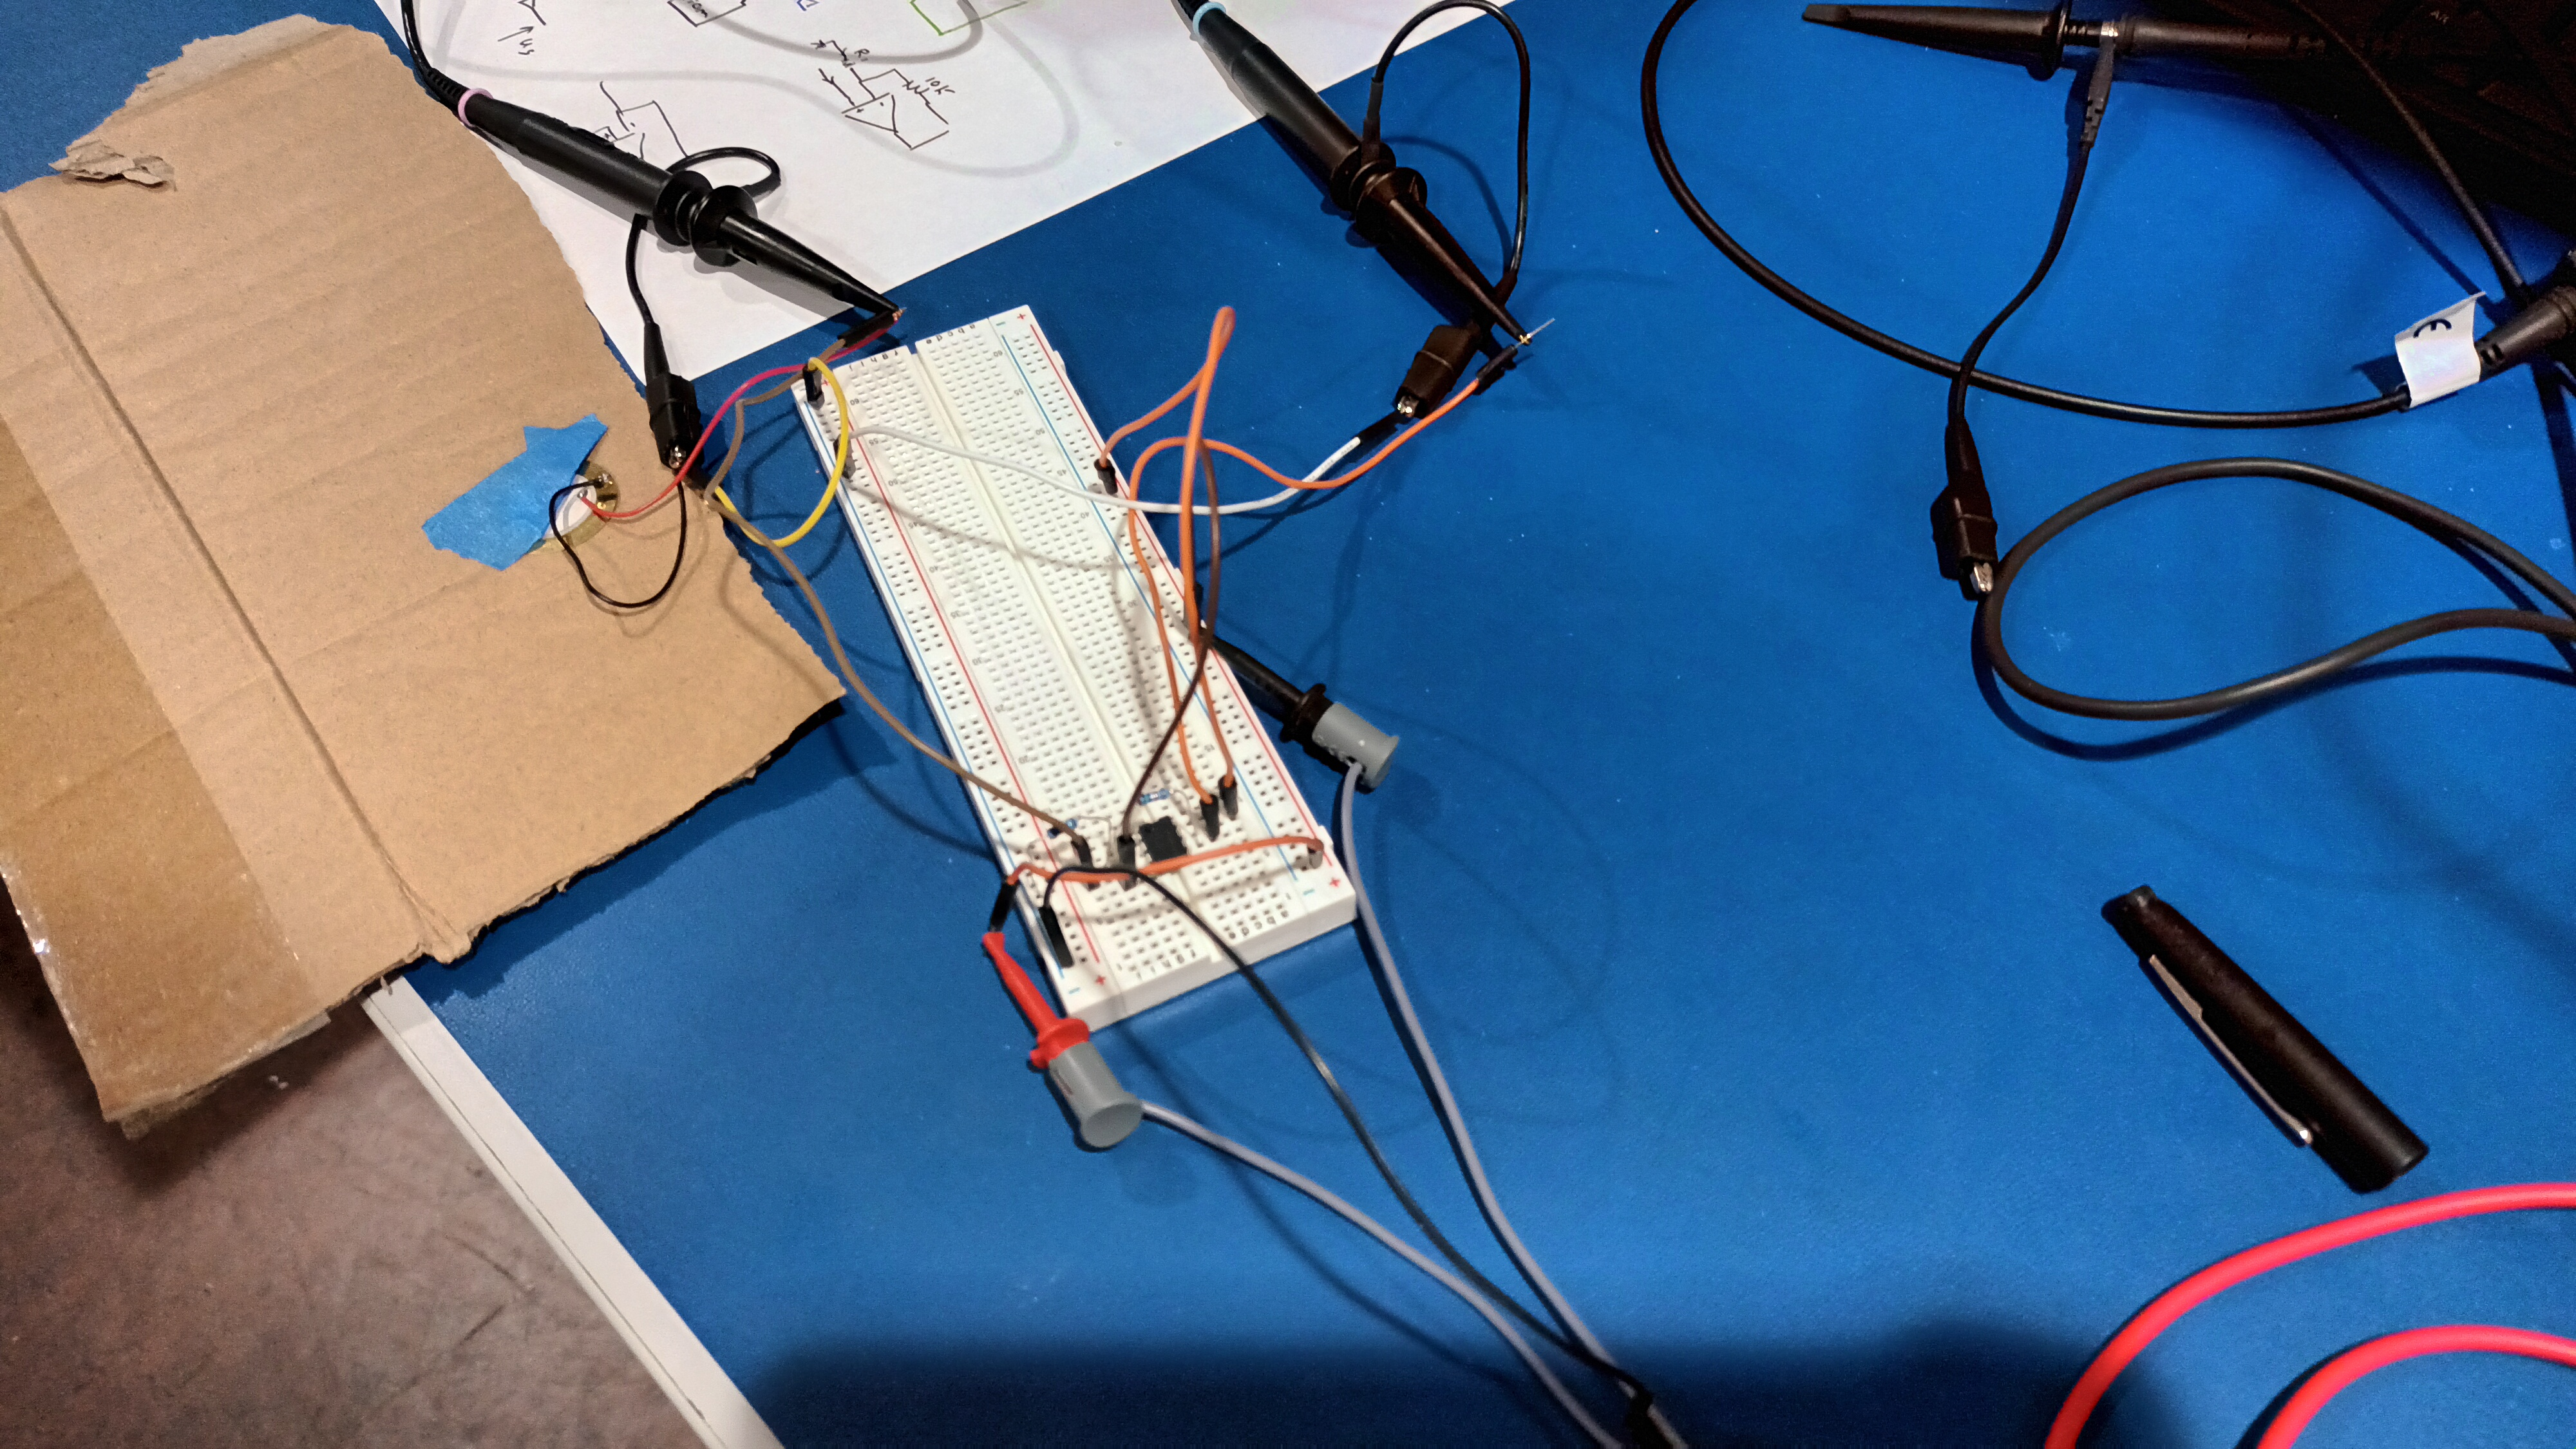
\includegraphics[scale=0.08]{montage_piezo_aop.jpg}
	\captionof{figure}{Montage piezo AOP }
	\label{image3}
	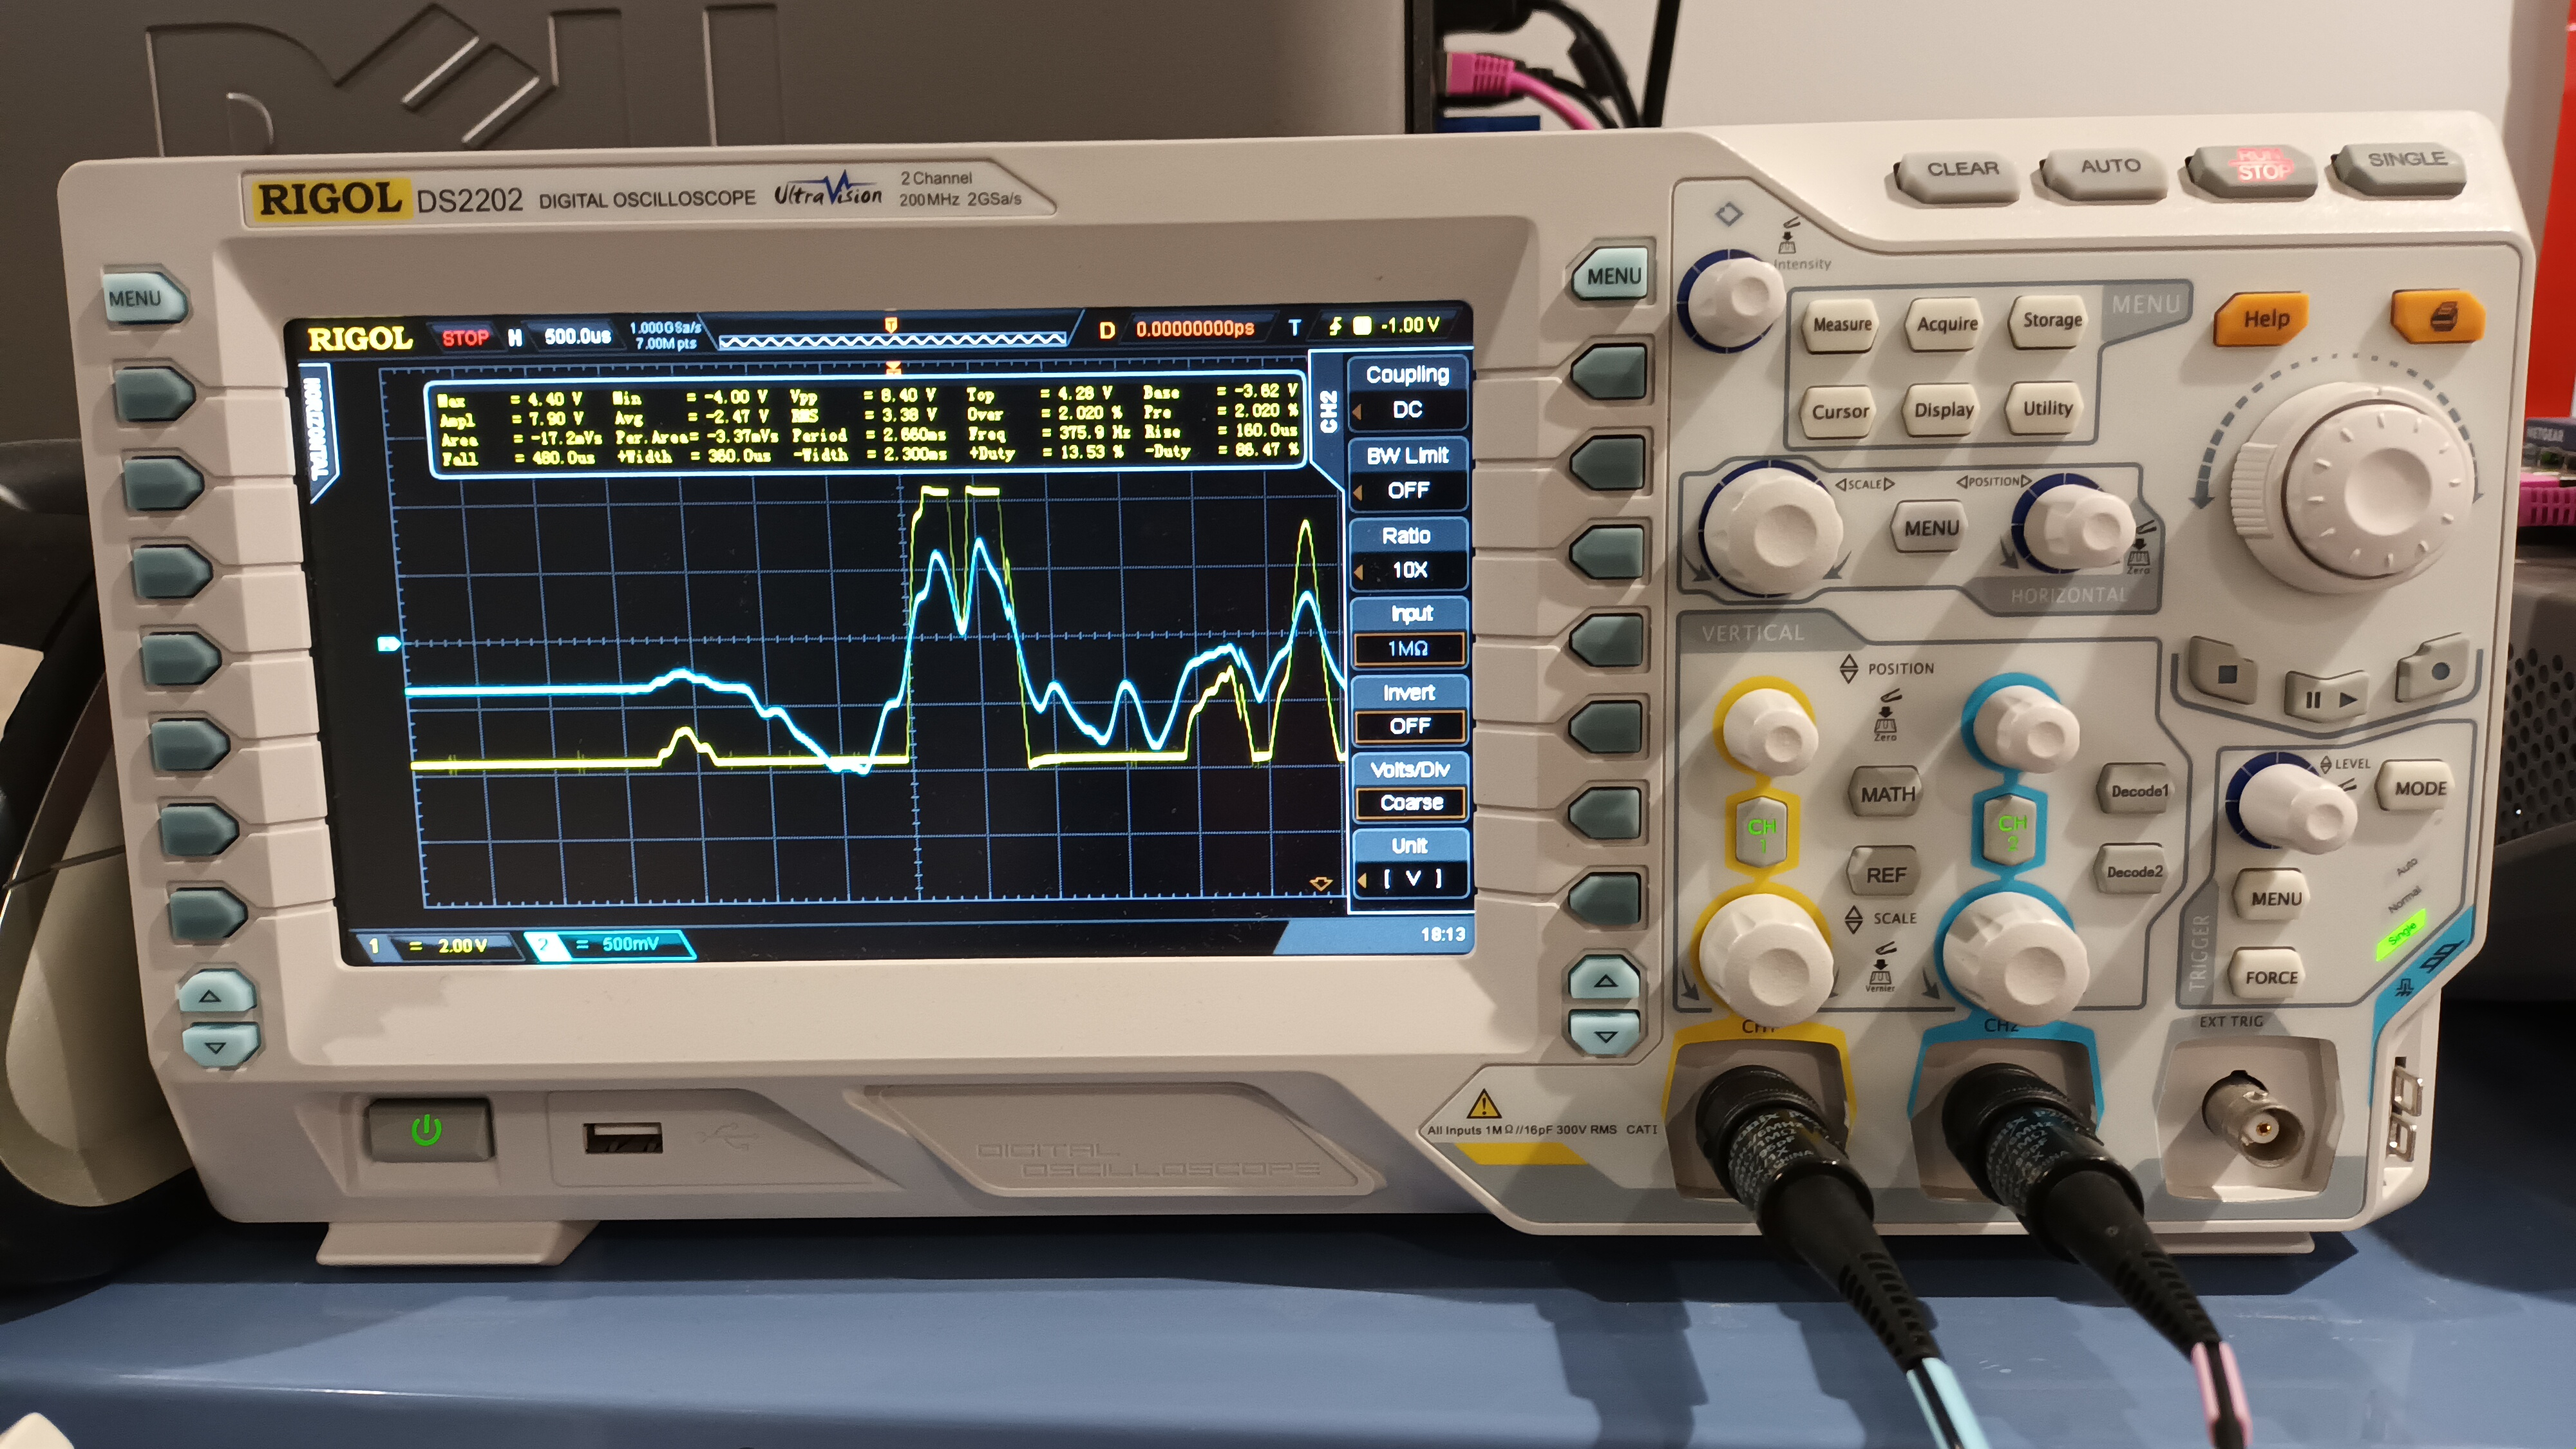
\includegraphics[scale=0.08]{sortie_osciloscope.jpg}
	\captionof{figure}{Comparatif post et pre amplification}
	\label{image4}
\end{center}
	
J'ai cependant rencontrer plusieur probleme sur le montage de l'AOP. Tout d'abords n'etants pas habituer 
a les manipuler j'ai confondue plusieur fois les differentes broches de cellui-ci. Ensuite le soucis manjeur 
c'est trouver aux niveaux de l'alimentation de cellui-ci. L'alimentation par les broche V- et V+ devais ce faire 
de manier cimetrique. 
Apres avoire solutioner tous ces probleme j'ai pu obtenire un premier montage fonctionnel.

\subsection{Liaisons des donner}
L'arduino et le shield ethernet sont fonctionnel et capable d'envoyer les donner recolter via MQTT.

\section{Travail a venire}
Mes objectif pour la semaine a venire sont les suivants :\\
	- Mieux comprendre les données recolte par le capteur piezo\\
	- Debuter l'etude du micro donner\\
	- Terminer le montage AOP d'instrumentation\\
	- Mettre des premier capteurs de temperature en fonctionment\\
	- Etudier le travail de Kristine Branson\\

\newpage
\listoffigures
\end{document}
